\documentclass[1p]{elsarticle_modified}
%\bibliographystyle{elsarticle-num}

%\usepackage[colorlinks]{hyperref}
%\usepackage{abbrmath_seonhwa} %\Abb, \Ascr, \Acal ,\Abf, \Afrak
\usepackage{amsfonts}
\usepackage{amssymb}
\usepackage{amsmath}
\usepackage{amsthm}
\usepackage{scalefnt}
\usepackage{amsbsy}
\usepackage{kotex}
\usepackage{caption}
\usepackage{subfig}
\usepackage{color}
\usepackage{graphicx}
\usepackage{xcolor} %% white, black, red, green, blue, cyan, magenta, yellow
\usepackage{float}
\usepackage{setspace}
\usepackage{hyperref}

\usepackage{tikz}
\usetikzlibrary{arrows}

\usepackage{multirow}
\usepackage{array} % fixed length table
\usepackage{hhline}

%%%%%%%%%%%%%%%%%%%%%
\makeatletter
\renewcommand*\env@matrix[1][\arraystretch]{%
	\edef\arraystretch{#1}%
	\hskip -\arraycolsep
	\let\@ifnextchar\new@ifnextchar
	\array{*\c@MaxMatrixCols c}}
\makeatother %https://tex.stackexchange.com/questions/14071/how-can-i-increase-the-line-spacing-in-a-matrix
%%%%%%%%%%%%%%%

\usepackage[normalem]{ulem}

\newcommand{\msout}[1]{\ifmmode\text{\sout{\ensuremath{#1}}}\else\sout{#1}\fi}
%SOURCE: \msout is \stkout macro in https://tex.stackexchange.com/questions/20609/strikeout-in-math-mode

\newcommand{\cancel}[1]{
	\ifmmode
	{\color{red}\msout{#1}}
	\else
	{\color{red}\sout{#1}}
	\fi
}

\newcommand{\add}[1]{
	{\color{blue}\uwave{#1}}
}

\newcommand{\replace}[2]{
	\ifmmode
	{\color{red}\msout{#1}}{\color{blue}\uwave{#2}}
	\else
	{\color{red}\sout{#1}}{\color{blue}\uwave{#2}}
	\fi
}

\newcommand{\Sol}{\mathcal{S}} %segment
\newcommand{\D}{D} %diagram
\newcommand{\A}{\mathcal{A}} %arc


%%%%%%%%%%%%%%%%%%%%%%%%%%%%%5 test

\def\sl{\operatorname{\textup{SL}}(2,\Cbb)}
\def\psl{\operatorname{\textup{PSL}}(2,\Cbb)}
\def\quan{\mkern 1mu \triangleright \mkern 1mu}

\theoremstyle{definition}
\newtheorem{thm}{Theorem}[section]
\newtheorem{prop}[thm]{Proposition}
\newtheorem{lem}[thm]{Lemma}
\newtheorem{ques}[thm]{Question}
\newtheorem{cor}[thm]{Corollary}
\newtheorem{defn}[thm]{Definition}
\newtheorem{exam}[thm]{Example}
\newtheorem{rmk}[thm]{Remark}
\newtheorem{alg}[thm]{Algorithm}

\newcommand{\I}{\sqrt{-1}}
\begin{document}

%\begin{frontmatter}
%
%\title{Boundary parabolic representations of knots up to 8 crossings}
%
%%% Group authors per affiliation:
%\author{Yunhi Cho} 
%\address{Department of Mathematics, University of Seoul, Seoul, Korea}
%\ead{yhcho@uos.ac.kr}
%
%
%\author{Seonhwa Kim} %\fnref{s_kim}}
%\address{Center for Geometry and Physics, Institute for Basic Science, Pohang, 37673, Korea}
%\ead{ryeona17@ibs.re.kr}
%
%\author{Hyuk Kim}
%\address{Department of Mathematical Sciences, Seoul National University, Seoul 08826, Korea}
%\ead{hyukkim@snu.ac.kr}
%
%\author{Seokbeom Yoon}
%\address{Department of Mathematical Sciences, Seoul National University, Seoul, 08826,  Korea}
%\ead{sbyoon15@snu.ac.kr}
%
%\begin{abstract}
%We find all boundary parabolic representation of knots up to 8 crossings.
%
%\end{abstract}
%\begin{keyword}
%    \MSC[2010] 57M25 
%\end{keyword}
%
%\end{frontmatter}

%\linenumbers
%\tableofcontents
%
\newcommand\colored[1]{\textcolor{white}{\rule[-0.35ex]{0.8em}{1.4ex}}\kern-0.8em\color{red} #1}%
%\newcommand\colored[1]{\textcolor{white}{ #1}\kern-2.17ex	\textcolor{white}{ #1}\kern-1.81ex	\textcolor{white}{ #1}\kern-2.15ex\color{red}#1	}

{\Large $\underline{12a_{0708}~(K12a_{0708})}$}

\setlength{\tabcolsep}{10pt}
\renewcommand{\arraystretch}{1.6}
\vspace{1cm}\begin{tabular}{m{100pt}>{\centering\arraybackslash}m{274pt}}
\multirow{5}{120pt}{
	\centering
	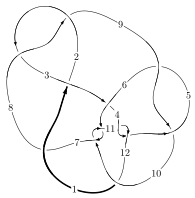
\includegraphics[width=112pt]{../../../GIT/diagram.site/Diagrams/png/1509_12a_0708.png}\\
\ \ \ A knot diagram\footnotemark}&
\allowdisplaybreaks
\textbf{Linearized knot diagam} \\
\cline{2-2}
 &
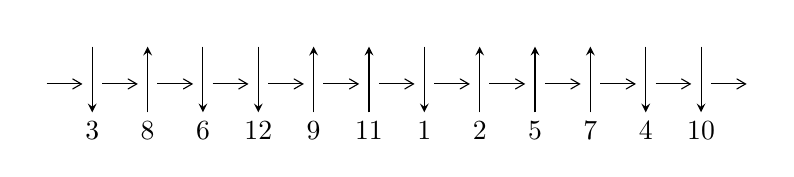
\begin{tikzpicture}[x=20pt, y=17pt]
	% nodes
	\node (C0) at (0, 0) {};
	\node (C1) at (1, 0) {};
	\node (C1U) at (1, +1) {};
	\node (C1D) at (1, -1) {3};

	\node (C2) at (2, 0) {};
	\node (C2U) at (2, +1) {};
	\node (C2D) at (2, -1) {8};

	\node (C3) at (3, 0) {};
	\node (C3U) at (3, +1) {};
	\node (C3D) at (3, -1) {6};

	\node (C4) at (4, 0) {};
	\node (C4U) at (4, +1) {};
	\node (C4D) at (4, -1) {12};

	\node (C5) at (5, 0) {};
	\node (C5U) at (5, +1) {};
	\node (C5D) at (5, -1) {9};

	\node (C6) at (6, 0) {};
	\node (C6U) at (6, +1) {};
	\node (C6D) at (6, -1) {11};

	\node (C7) at (7, 0) {};
	\node (C7U) at (7, +1) {};
	\node (C7D) at (7, -1) {1};

	\node (C8) at (8, 0) {};
	\node (C8U) at (8, +1) {};
	\node (C8D) at (8, -1) {2};

	\node (C9) at (9, 0) {};
	\node (C9U) at (9, +1) {};
	\node (C9D) at (9, -1) {5};

	\node (C10) at (10, 0) {};
	\node (C10U) at (10, +1) {};
	\node (C10D) at (10, -1) {7};

	\node (C11) at (11, 0) {};
	\node (C11U) at (11, +1) {};
	\node (C11D) at (11, -1) {4};

	\node (C12) at (12, 0) {};
	\node (C12U) at (12, +1) {};
	\node (C12D) at (12, -1) {10};
	\node (C13) at (13, 0) {};

	% arrows
	\draw[->,>={angle 60}]
	(C0) edge (C1) (C1) edge (C2) (C2) edge (C3) (C3) edge (C4) (C4) edge (C5) (C5) edge (C6) (C6) edge (C7) (C7) edge (C8) (C8) edge (C9) (C9) edge (C10) (C10) edge (C11) (C11) edge (C12) (C12) edge (C13) ;	\draw[->,>=stealth]
	(C1U) edge (C1D) (C2D) edge (C2U) (C3U) edge (C3D) (C4U) edge (C4D) (C5D) edge (C5U) (C6D) edge (C6U) (C7U) edge (C7D) (C8D) edge (C8U) (C9D) edge (C9U) (C10D) edge (C10U) (C11U) edge (C11D) (C12U) edge (C12D) ;
	\end{tikzpicture} \\
\hhline{~~} \\& 
\textbf{Solving Sequence} \\ \cline{2-2} 
 &
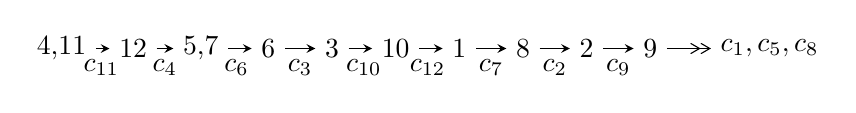
\begin{tikzpicture}[x=23pt, y=7pt]
	% node
	\node (A0) at (-1/8, 0) {4,11};
	\node (A1) at (1, 0) {12};
	\node (A2) at (33/16, 0) {5,7};
	\node (A3) at (25/8, 0) {6};
	\node (A4) at (33/8, 0) {3};
	\node (A5) at (41/8, 0) {10};
	\node (A6) at (49/8, 0) {1};
	\node (A7) at (57/8, 0) {8};
	\node (A8) at (65/8, 0) {2};
	\node (A9) at (73/8, 0) {9};
	\node (C1) at (1/2, -1) {$c_{11}$};
	\node (C2) at (3/2, -1) {$c_{4}$};
	\node (C3) at (21/8, -1) {$c_{6}$};
	\node (C4) at (29/8, -1) {$c_{3}$};
	\node (C5) at (37/8, -1) {$c_{10}$};
	\node (C6) at (45/8, -1) {$c_{12}$};
	\node (C7) at (53/8, -1) {$c_{7}$};
	\node (C8) at (61/8, -1) {$c_{2}$};
	\node (C9) at (69/8, -1) {$c_{9}$};
	\node (A10) at (11, 0) {$c_{1},c_{5},c_{8}$};

	% edge
	\draw[->,>=stealth]	
	(A0) edge (A1) (A1) edge (A2) (A2) edge (A3) (A3) edge (A4) (A4) edge (A5) (A5) edge (A6) (A6) edge (A7) (A7) edge (A8) (A8) edge (A9) ;
	\draw[->>,>={angle 60}]	
	(A9) edge (A10);
\end{tikzpicture} \\ 

\end{tabular} \\

\footnotetext{
The image of knot diagram is generated by the software ``\textbf{Draw programme}" developed by Andrew Bartholomew(\url{http://www.layer8.co.uk/maths/draw/index.htm\#Running-draw}), where we modified some parts for our purpose(\url{https://github.com/CATsTAILs/LinksPainter}).
}\phantom \\ \newline 
\centering \textbf{Ideals for irreducible components\footnotemark of $X_{\text{par}}$} 
 
\begin{align*}
I^u_{1}&=\langle 
-1.09180\times10^{106} u^{45}+2.54989\times10^{106} u^{44}+\cdots+1.47540\times10^{109} b-9.66672\times10^{108},\\
\phantom{I^u_{1}}&\phantom{= \langle  }-3.14133\times10^{108} u^{45}+6.29434\times10^{108} u^{44}+\cdots+5.90159\times10^{110} a-2.38197\times10^{111},\\
\phantom{I^u_{1}}&\phantom{= \langle  }u^{46}-2 u^{45}+\cdots+841 u-160\rangle \\
I^u_{2}&=\langle 
u^{31}- u^{30}+\cdots+a+2,\;2 u^{31} a+4 u^{31}+\cdots+6 a+4,\;u^{32}- u^{31}+\cdots+2 u-1\rangle \\
I^u_{3}&=\langle 
b+1,\;16 a^4+32 a^3+16 a^2+1,\;u+1\rangle \\
I^u_{4}&=\langle 
2 u^2 a- a u+3 u^2+b+2 a- u+5,\;70 u^2 a+25 a^2-40 a u+91 u^2+130 a-42 u+169,\;u^3- u^2+2 u-1\rangle \\
I^u_{5}&=\langle 
b-1,\;8 a^3-12 a^2+6 a-1,\;u-1\rangle \\
\\
\end{align*}
\raggedright * 5 irreducible components of $\dim_{\mathbb{C}}=0$, with total 123 representations.\\
\footnotetext{All coefficients of polynomials are rational numbers. But the coefficients are sometimes approximated in decimal forms when there is not enough margin.}
\newpage
\renewcommand{\arraystretch}{1}
\centering \section*{I. $I^u_{1}= \langle -1.09\times10^{106} u^{45}+2.55\times10^{106} u^{44}+\cdots+1.48\times10^{109} b-9.67\times10^{108},\;-3.14\times10^{108} u^{45}+6.29\times10^{108} u^{44}+\cdots+5.90\times10^{110} a-2.38\times10^{111},\;u^{46}-2 u^{45}+\cdots+841 u-160 \rangle$}
\flushleft \textbf{(i) Arc colorings}\\
\begin{tabular}{m{7pt} m{180pt} m{7pt} m{180pt} }
\flushright $a_{4}=$&$\begin{pmatrix}0\\u\end{pmatrix}$ \\
\flushright $a_{11}=$&$\begin{pmatrix}1\\0\end{pmatrix}$ \\
\flushright $a_{12}=$&$\begin{pmatrix}1\\u^2\end{pmatrix}$ \\
\flushright $a_{5}=$&$\begin{pmatrix}- u\\- u^3+u\end{pmatrix}$ \\
\flushright $a_{7}=$&$\begin{pmatrix}0.00532285 u^{45}-0.0106655 u^{44}+\cdots-6.13310 u+4.03615\\0.000740005 u^{45}-0.00172827 u^{44}+\cdots+1.78965 u+0.655195\end{pmatrix}$ \\
\flushright $a_{6}=$&$\begin{pmatrix}0.00458285 u^{45}-0.00893723 u^{44}+\cdots-7.92275 u+3.38096\\0.000740005 u^{45}-0.00172827 u^{44}+\cdots+1.78965 u+0.655195\end{pmatrix}$ \\
\flushright $a_{3}=$&$\begin{pmatrix}0.00266979 u^{45}-0.00467810 u^{44}+\cdots-7.89898 u+1.66017\\0.000649223 u^{45}-0.00112824 u^{44}+\cdots+0.509083 u+0.599334\end{pmatrix}$ \\
\flushright $a_{10}=$&$\begin{pmatrix}0.00386651 u^{45}-0.00706006 u^{44}+\cdots-7.67006 u+4.50026\\0.000120669 u^{45}-0.000217602 u^{44}+\cdots-0.420533 u+0.840929\end{pmatrix}$ \\
\flushright $a_{1}=$&$\begin{pmatrix}0.00308435 u^{45}-0.00557645 u^{44}+\cdots-6.66439 u+3.23217\\0.000567357 u^{45}-0.00102442 u^{44}+\cdots-0.589724 u+0.521928\end{pmatrix}$ \\
\flushright $a_{8}=$&$\begin{pmatrix}0.000163084 u^{45}-0.000998201 u^{44}+\cdots+4.27507 u+0.948641\\-0.000225587 u^{45}-0.000445073 u^{44}+\cdots+3.77056 u-0.0255609\end{pmatrix}$ \\
\flushright $a_{2}=$&$\begin{pmatrix}0.00488531 u^{45}-0.00821426 u^{44}+\cdots-15.9169 u+3.03609\\0.00128027 u^{45}-0.00211403 u^{44}+\cdots-2.99501 u+1.51400\end{pmatrix}$ \\
\flushright $a_{9}=$&$\begin{pmatrix}0.00411477 u^{45}-0.00750092 u^{44}+\cdots-7.70291 u+4.38186\\0.000191354 u^{45}-0.000279609 u^{44}+\cdots-0.394775 u+0.968236\end{pmatrix}$\\&\end{tabular}
\flushleft \textbf{(ii) Obstruction class $= -1$}\\~\\
\flushleft \textbf{(iii) Cusp Shapes $= 0.00201846 u^{45}-0.00557907 u^{44}+\cdots-13.0415 u+5.45038$}\\~\\
\newpage\renewcommand{\arraystretch}{1}
\flushleft \textbf{(iv) u-Polynomials at the component}\newline \\
\begin{tabular}{m{50pt}|m{274pt}}
Crossings & \hspace{64pt}u-Polynomials at each crossing \\
\hline $$\begin{aligned}c_{1}\end{aligned}$$&$\begin{aligned}
&u^{46}+23 u^{45}+\cdots+112 u+64
\end{aligned}$\\
\hline $$\begin{aligned}c_{2},c_{8}\end{aligned}$$&$\begin{aligned}
&u^{46}+3 u^{45}+\cdots+28 u+8
\end{aligned}$\\
\hline $$\begin{aligned}c_{3},c_{12}\end{aligned}$$&$\begin{aligned}
&128(128 u^{46}-576 u^{45}+\cdots-9 u+1)
\end{aligned}$\\
\hline $$\begin{aligned}c_{4},c_{11}\end{aligned}$$&$\begin{aligned}
&u^{46}+2 u^{45}+\cdots-841 u-160
\end{aligned}$\\
\hline $$\begin{aligned}c_{5},c_{6},c_{9}\\c_{10}\end{aligned}$$&$\begin{aligned}
&u^{46}+u^{45}+\cdots-14 u-1
\end{aligned}$\\
\hline $$\begin{aligned}c_{7}\end{aligned}$$&$\begin{aligned}
&u^{46}-3 u^{45}+\cdots-24020 u+12872
\end{aligned}$\\
\hline
\end{tabular}\\~\\
\newpage\renewcommand{\arraystretch}{1}
\flushleft \textbf{(v) Riley Polynomials at the component}\newline \\
\begin{tabular}{m{50pt}|m{274pt}}
Crossings & \hspace{64pt}Riley Polynomials at each crossing \\
\hline $$\begin{aligned}c_{1}\end{aligned}$$&$\begin{aligned}
&y^{46}+3 y^{45}+\cdots-45312 y+4096
\end{aligned}$\\
\hline $$\begin{aligned}c_{2},c_{8}\end{aligned}$$&$\begin{aligned}
&y^{46}+23 y^{45}+\cdots+112 y+64
\end{aligned}$\\
\hline $$\begin{aligned}c_{3},c_{12}\end{aligned}$$&$\begin{aligned}
&16384(16384 y^{46}-569344 y^{45}+\cdots-97 y+1)
\end{aligned}$\\
\hline $$\begin{aligned}c_{4},c_{11}\end{aligned}$$&$\begin{aligned}
&y^{46}-28 y^{45}+\cdots-649361 y+25600
\end{aligned}$\\
\hline $$\begin{aligned}c_{5},c_{6},c_{9}\\c_{10}\end{aligned}$$&$\begin{aligned}
&y^{46}+31 y^{45}+\cdots+78 y+1
\end{aligned}$\\
\hline $$\begin{aligned}c_{7}\end{aligned}$$&$\begin{aligned}
&y^{46}-17 y^{45}+\cdots+1347455088 y+165688384
\end{aligned}$\\
\hline
\end{tabular}\\~\\
\newpage\flushleft \textbf{(vi) Complex Volumes and Cusp Shapes}
$$\begin{array}{c|c|c}  
\text{Solutions to }I^u_{1}& \I (\text{vol} + \sqrt{-1}CS) & \text{Cusp shape}\\
 \hline 
\begin{aligned}
u &= \phantom{-}0.966769 + 0.336158 I \\
a &= \phantom{-}0.487792 + 0.360103 I \\
b &= \phantom{-}0.823732 + 0.567954 I\end{aligned}
 & -1.06197 + 2.22747 I & -2.33539 - 2.53265 I \\ \hline\begin{aligned}
u &= \phantom{-}0.966769 - 0.336158 I \\
a &= \phantom{-}0.487792 - 0.360103 I \\
b &= \phantom{-}0.823732 - 0.567954 I\end{aligned}
 & -1.06197 - 2.22747 I & -2.33539 + 2.53265 I \\ \hline\begin{aligned}
u &= -1.022710 + 0.054575 I \\
a &= \phantom{-}1.065410 - 0.295918 I \\
b &= \phantom{-}0.0351231 - 0.1143600 I\end{aligned}
 & -4.15103 + 3.62905 I & -9.89130 - 4.16048 I \\ \hline\begin{aligned}
u &= -1.022710 - 0.054575 I \\
a &= \phantom{-}1.065410 + 0.295918 I \\
b &= \phantom{-}0.0351231 + 0.1143600 I\end{aligned}
 & -4.15103 - 3.62905 I & -9.89130 + 4.16048 I \\ \hline\begin{aligned}
u &= \phantom{-}0.300795 + 1.016240 I \\
a &= \phantom{-}0.098981 + 0.607252 I \\
b &= \phantom{-}0.114437 + 0.723964 I\end{aligned}
 & \phantom{-}0.64788 - 2.52803 I & \phantom{-}4.19226 + 0.68863 I \\ \hline\begin{aligned}
u &= \phantom{-}0.300795 - 1.016240 I \\
a &= \phantom{-}0.098981 - 0.607252 I \\
b &= \phantom{-}0.114437 - 0.723964 I\end{aligned}
 & \phantom{-}0.64788 + 2.52803 I & \phantom{-}4.19226 - 0.68863 I \\ \hline\begin{aligned}
u &= \phantom{-}0.920916\phantom{ +0.000000I} \\
a &= -0.662681\phantom{ +0.000000I} \\
b &= \phantom{-}0.145994\phantom{ +0.000000I}\end{aligned}
 & -1.48897\phantom{ +0.000000I} & -6.56270\phantom{ +0.000000I} \\ \hline\begin{aligned}
u &= -1.089920 + 0.144544 I \\
a &= -0.610206 + 0.169024 I \\
b &= -1.154580 + 0.317622 I\end{aligned}
 & -0.053677 + 0.799227 I & -3.87957 - 8.61272 I \\ \hline\begin{aligned}
u &= -1.089920 - 0.144544 I \\
a &= -0.610206 - 0.169024 I \\
b &= -1.154580 - 0.317622 I\end{aligned}
 & -0.053677 - 0.799227 I & -3.87957 + 8.61272 I \\ \hline\begin{aligned}
u &= \phantom{-}0.830377 + 0.297025 I \\
a &= -0.408161 - 0.736370 I \\
b &= \phantom{-}0.270178 - 0.394032 I\end{aligned}
 & -1.84309 - 0.93078 I & -5.79685 + 4.30580 I\\
 \hline 
 \end{array}$$\newpage$$\begin{array}{c|c|c}  
\text{Solutions to }I^u_{1}& \I (\text{vol} + \sqrt{-1}CS) & \text{Cusp shape}\\
 \hline 
\begin{aligned}
u &= \phantom{-}0.830377 - 0.297025 I \\
a &= -0.408161 + 0.736370 I \\
b &= \phantom{-}0.270178 + 0.394032 I\end{aligned}
 & -1.84309 + 0.93078 I & -5.79685 - 4.30580 I \\ \hline\begin{aligned}
u &= -1.20992\phantom{ +0.000000I} \\
a &= -0.752195\phantom{ +0.000000I} \\
b &= -1.48735\phantom{ +0.000000I}\end{aligned}
 & -1.03932\phantom{ +0.000000I} & -8.02530\phantom{ +0.000000I} \\ \hline\begin{aligned}
u &= \phantom{-}0.467930 + 0.629000 I \\
a &= -0.488824 - 1.031510 I \\
b &= \phantom{-}0.576714 - 0.673740 I\end{aligned}
 & \phantom{-}0.40716 - 5.93075 I & \phantom{-}1.20971 + 10.32229 I \\ \hline\begin{aligned}
u &= \phantom{-}0.467930 - 0.629000 I \\
a &= -0.488824 + 1.031510 I \\
b &= \phantom{-}0.576714 + 0.673740 I\end{aligned}
 & \phantom{-}0.40716 + 5.93075 I & \phantom{-}1.20971 - 10.32229 I \\ \hline\begin{aligned}
u &= \phantom{-}1.256000 + 0.034981 I \\
a &= \phantom{-}0.807767 + 0.042667 I \\
b &= \phantom{-}1.61598 + 0.10458 I\end{aligned}
 & -4.20433 - 4.10865 I & -10.31107 + 4.30154 I \\ \hline\begin{aligned}
u &= \phantom{-}1.256000 - 0.034981 I \\
a &= \phantom{-}0.807767 - 0.042667 I \\
b &= \phantom{-}1.61598 - 0.10458 I\end{aligned}
 & -4.20433 + 4.10865 I & -10.31107 - 4.30154 I \\ \hline\begin{aligned}
u &= -0.196424 + 1.258430 I \\
a &= \phantom{-}0.327145 - 0.489998 I \\
b &= -0.372089 - 1.349360 I\end{aligned}
 & -9.1285 + 12.2286 I & -6.60036 - 8.01621 I \\ \hline\begin{aligned}
u &= -0.196424 - 1.258430 I \\
a &= \phantom{-}0.327145 + 0.489998 I \\
b &= -0.372089 + 1.349360 I\end{aligned}
 & -9.1285 - 12.2286 I & -6.60036 + 8.01621 I \\ \hline\begin{aligned}
u &= \phantom{-}0.226130 + 1.306880 I \\
a &= -0.283030 - 0.536087 I \\
b &= \phantom{-}0.311390 - 1.307260 I\end{aligned}
 & -6.02382 - 6.82285 I & -4.45743 + 5.16086 I \\ \hline\begin{aligned}
u &= \phantom{-}0.226130 - 1.306880 I \\
a &= -0.283030 + 0.536087 I \\
b &= \phantom{-}0.311390 + 1.307260 I\end{aligned}
 & -6.02382 + 6.82285 I & -4.45743 - 5.16086 I\\
 \hline 
 \end{array}$$\newpage$$\begin{array}{c|c|c}  
\text{Solutions to }I^u_{1}& \I (\text{vol} + \sqrt{-1}CS) & \text{Cusp shape}\\
 \hline 
\begin{aligned}
u &= -0.152157 + 1.357930 I \\
a &= \phantom{-}0.196395 - 0.491844 I \\
b &= -0.222197 - 1.374140 I\end{aligned}
 & -10.97740 + 2.63730 I & -9.44645 - 2.07014 I \\ \hline\begin{aligned}
u &= -0.152157 - 1.357930 I \\
a &= \phantom{-}0.196395 + 0.491844 I \\
b &= -0.222197 + 1.374140 I\end{aligned}
 & -10.97740 - 2.63730 I & -9.44645 + 2.07014 I \\ \hline\begin{aligned}
u &= -0.415745 + 0.454460 I \\
a &= \phantom{-}0.339820 - 1.213850 I \\
b &= -0.630617 - 0.516212 I\end{aligned}
 & \phantom{-}1.71362 + 1.56853 I & \phantom{-}5.64296 - 4.27493 I \\ \hline\begin{aligned}
u &= -0.415745 - 0.454460 I \\
a &= \phantom{-}0.339820 + 1.213850 I \\
b &= -0.630617 + 0.516212 I\end{aligned}
 & \phantom{-}1.71362 - 1.56853 I & \phantom{-}5.64296 + 4.27493 I \\ \hline\begin{aligned}
u &= \phantom{-}1.47895 + 0.51753 I \\
a &= \phantom{-}0.69888 + 1.63660 I \\
b &= -0.55966 + 1.47409 I\end{aligned}
 & -14.4351 - 18.4106 I & \phantom{-0.000000 } 0 \\ \hline\begin{aligned}
u &= \phantom{-}1.47895 - 0.51753 I \\
a &= \phantom{-}0.69888 - 1.63660 I \\
b &= -0.55966 - 1.47409 I\end{aligned}
 & -14.4351 + 18.4106 I & \phantom{-0.000000 } 0 \\ \hline\begin{aligned}
u &= -1.49451 + 0.51469 I \\
a &= -0.66292 + 1.61664 I \\
b &= \phantom{-}0.51926 + 1.45348 I\end{aligned}
 & -11.4919 + 13.1095 I & \phantom{-0.000000 } 0 \\ \hline\begin{aligned}
u &= -1.49451 - 0.51469 I \\
a &= -0.66292 - 1.61664 I \\
b &= \phantom{-}0.51926 - 1.45348 I\end{aligned}
 & -11.4919 - 13.1095 I & \phantom{-0.000000 } 0 \\ \hline\begin{aligned}
u &= \phantom{-}1.50459 + 0.53805 I \\
a &= \phantom{-}0.67757 + 1.55296 I \\
b &= -0.46575 + 1.50413 I\end{aligned}
 & -16.3159 - 9.1985 I & \phantom{-0.000000 } 0 \\ \hline\begin{aligned}
u &= \phantom{-}1.50459 - 0.53805 I \\
a &= \phantom{-}0.67757 - 1.55296 I \\
b &= -0.46575 - 1.50413 I\end{aligned}
 & -16.3159 + 9.1985 I & \phantom{-0.000000 } 0\\
 \hline 
 \end{array}$$\newpage$$\begin{array}{c|c|c}  
\text{Solutions to }I^u_{1}& \I (\text{vol} + \sqrt{-1}CS) & \text{Cusp shape}\\
 \hline 
\begin{aligned}
u &= -0.319923 + 0.205407 I \\
a &= -0.49892 - 1.47670 I \\
b &= -0.684519 - 0.269684 I\end{aligned}
 & \phantom{-}1.299950 + 0.545169 I & \phantom{-}7.33327 - 2.66356 I \\ \hline\begin{aligned}
u &= -0.319923 - 0.205407 I \\
a &= -0.49892 + 1.47670 I \\
b &= -0.684519 + 0.269684 I\end{aligned}
 & \phantom{-}1.299950 - 0.545169 I & \phantom{-}7.33327 + 2.66356 I \\ \hline\begin{aligned}
u &= -1.58193 + 0.48587 I \\
a &= -0.47480 + 1.54895 I \\
b &= \phantom{-}0.375465 + 1.314860 I\end{aligned}
 & -7.50745 + 10.56620 I & \phantom{-0.000000 } 0 \\ \hline\begin{aligned}
u &= -1.58193 - 0.48587 I \\
a &= -0.47480 - 1.54895 I \\
b &= \phantom{-}0.375465 - 1.314860 I\end{aligned}
 & -7.50745 - 10.56620 I & \phantom{-0.000000 } 0 \\ \hline\begin{aligned}
u &= -1.58450 + 0.64719 I \\
a &= -0.554722 + 1.269070 I \\
b &= \phantom{-}0.10580 + 1.45206 I\end{aligned}
 & -15.5466 + 4.8809 I & \phantom{-0.000000 } 0 \\ \hline\begin{aligned}
u &= -1.58450 - 0.64719 I \\
a &= -0.554722 - 1.269070 I \\
b &= \phantom{-}0.10580 - 1.45206 I\end{aligned}
 & -15.5466 - 4.8809 I & \phantom{-0.000000 } 0 \\ \hline\begin{aligned}
u &= \phantom{-}0.10957 + 1.71612 I \\
a &= -0.044906 - 0.687293 I \\
b &= \phantom{-}0.041280 - 1.188470 I\end{aligned}
 & -1.28695 - 3.16258 I & \phantom{-0.000000 } 0 \\ \hline\begin{aligned}
u &= \phantom{-}0.10957 - 1.71612 I \\
a &= -0.044906 + 0.687293 I \\
b &= \phantom{-}0.041280 + 1.188470 I\end{aligned}
 & -1.28695 + 3.16258 I & \phantom{-0.000000 } 0 \\ \hline\begin{aligned}
u &= \phantom{-}1.64163 + 0.51374 I \\
a &= \phantom{-}0.42138 + 1.45572 I \\
b &= -0.280308 + 1.292080 I\end{aligned}
 & -7.10146 - 4.90994 I & \phantom{-0.000000 } 0 \\ \hline\begin{aligned}
u &= \phantom{-}1.64163 - 0.51374 I \\
a &= \phantom{-}0.42138 - 1.45572 I \\
b &= -0.280308 - 1.292080 I\end{aligned}
 & -7.10146 + 4.90994 I & \phantom{-0.000000 } 0\\
 \hline 
 \end{array}$$\newpage$$\begin{array}{c|c|c}  
\text{Solutions to }I^u_{1}& \I (\text{vol} + \sqrt{-1}CS) & \text{Cusp shape}\\
 \hline 
\begin{aligned}
u &= -1.56809 + 0.75350 I \\
a &= -0.505362 + 1.120240 I \\
b &= -0.063645 + 1.376890 I\end{aligned}
 & -13.07240 - 4.75404 I & \phantom{-0.000000 } 0 \\ \hline\begin{aligned}
u &= -1.56809 - 0.75350 I \\
a &= -0.505362 - 1.120240 I \\
b &= -0.063645 - 1.376890 I\end{aligned}
 & -13.07240 + 4.75404 I & \phantom{-0.000000 } 0 \\ \hline\begin{aligned}
u &= \phantom{-}1.62673 + 0.71859 I \\
a &= \phantom{-}0.469280 + 1.190400 I \\
b &= -0.021734 + 1.350920 I\end{aligned}
 & -10.16390 - 0.95021 I & \phantom{-0.000000 } 0 \\ \hline\begin{aligned}
u &= \phantom{-}1.62673 - 0.71859 I \\
a &= \phantom{-}0.469280 - 1.190400 I \\
b &= -0.021734 - 1.350920 I\end{aligned}
 & -10.16390 + 0.95021 I & \phantom{-0.000000 } 0 \\ \hline\begin{aligned}
u &= \phantom{-}0.160935 + 0.124811 I \\
a &= \phantom{-}2.02700 - 2.96588 I \\
b &= \phantom{-}0.836429 - 0.145266 I\end{aligned}
 & -0.85613 + 3.53276 I & \phantom{-}2.89113 - 3.11148 I \\ \hline\begin{aligned}
u &= \phantom{-}0.160935 - 0.124811 I \\
a &= \phantom{-}2.02700 + 2.96588 I \\
b &= \phantom{-}0.836429 + 0.145266 I\end{aligned}
 & -0.85613 - 3.53276 I & \phantom{-}2.89113 + 3.11148 I\\
 \hline 
 \end{array}$$\newpage\newpage\renewcommand{\arraystretch}{1}
\centering \section*{II. $I^u_{2}= \langle u^{31}- u^{30}+\cdots+a+2,\;2 u^{31} a+4 u^{31}+\cdots+6 a+4,\;u^{32}- u^{31}+\cdots+2 u-1 \rangle$}
\flushleft \textbf{(i) Arc colorings}\\
\begin{tabular}{m{7pt} m{180pt} m{7pt} m{180pt} }
\flushright $a_{4}=$&$\begin{pmatrix}0\\u\end{pmatrix}$ \\
\flushright $a_{11}=$&$\begin{pmatrix}1\\0\end{pmatrix}$ \\
\flushright $a_{12}=$&$\begin{pmatrix}1\\u^2\end{pmatrix}$ \\
\flushright $a_{5}=$&$\begin{pmatrix}- u\\- u^3+u\end{pmatrix}$ \\
\flushright $a_{7}=$&$\begin{pmatrix}a\\- u^{31}+u^{30}+\cdots- a-2\end{pmatrix}$ \\
\flushright $a_{6}=$&$\begin{pmatrix}u^{31}- u^{30}+\cdots+2 a+2\\- u^{31}+u^{30}+\cdots- a-2\end{pmatrix}$ \\
\flushright $a_{3}=$&$\begin{pmatrix}-2 u^{31} a- u^{31}+\cdots-4 a-12\\u^{31}+u^{30}+\cdots+a+4\end{pmatrix}$ \\
\flushright $a_{10}=$&$\begin{pmatrix}u^{31} a+4 u^{31}+\cdots+2 a+6\\- u^5 a- u^6+2 u^3 a+2 u^4- a u-2\end{pmatrix}$ \\
\flushright $a_{1}=$&$\begin{pmatrix}- u^{31} a-6 u^{31}+\cdots-4 a-6\\2 u^{31}-2 u^{30}+\cdots+2 u+4\end{pmatrix}$ \\
\flushright $a_{8}=$&$\begin{pmatrix}-2 u^{31} a+u^{31}+\cdots+8 u-8\\- u^{31}+3 u^{30}+\cdots- a+2 u\end{pmatrix}$ \\
\flushright $a_{2}=$&$\begin{pmatrix}- u^{31} a+u^{30} a+\cdots-2 a-11\\u^{23} a+u^{24}+\cdots+4 a u+5\end{pmatrix}$ \\
\flushright $a_{9}=$&$\begin{pmatrix}u^{31} a+4 u^{31}+\cdots+2 a+5\\-1\end{pmatrix}$\\&\end{tabular}
\flushleft \textbf{(ii) Obstruction class $= -1$}\\~\\
\flushleft \textbf{(iii) Cusp Shapes $= 4 u^{29}-48 u^{27}-4 u^{26}+252 u^{25}+44 u^{24}-740 u^{23}-208 u^{22}+1264 u^{21}+536 u^{20}-1080 u^{19}-768 u^{18}-64 u^{17}+480 u^{16}+1008 u^{15}+176 u^{14}-612 u^{13}-436 u^{12}-320 u^{11}+120 u^{10}+424 u^9+128 u^8+4 u^7-60 u^6-108 u^5-12 u^4+4 u^3+4 u^2+12 u-6$}\\~\\
\newpage\renewcommand{\arraystretch}{1}
\flushleft \textbf{(iv) u-Polynomials at the component}\newline \\
\begin{tabular}{m{50pt}|m{274pt}}
Crossings & \hspace{64pt}u-Polynomials at each crossing \\
\hline $$\begin{aligned}c_{1}\end{aligned}$$&$\begin{aligned}
&(u^{32}+17 u^{31}+\cdots-8 u^2+1)^{2}
\end{aligned}$\\
\hline $$\begin{aligned}c_{2},c_{8}\end{aligned}$$&$\begin{aligned}
&(u^{32}- u^{31}+\cdots+2 u-1)^{2}
\end{aligned}$\\
\hline $$\begin{aligned}c_{3},c_{12}\end{aligned}$$&$\begin{aligned}
&u^{64}+9 u^{63}+\cdots-753639276 u+67447447
\end{aligned}$\\
\hline $$\begin{aligned}c_{4},c_{11}\end{aligned}$$&$\begin{aligned}
&(u^{32}+u^{31}+\cdots-2 u-1)^{2}
\end{aligned}$\\
\hline $$\begin{aligned}c_{5},c_{6},c_{9}\\c_{10}\end{aligned}$$&$\begin{aligned}
&u^{64}-3 u^{63}+\cdots-588 u+173
\end{aligned}$\\
\hline $$\begin{aligned}c_{7}\end{aligned}$$&$\begin{aligned}
&(u^{32}+u^{31}+\cdots-14 u-5)^{2}
\end{aligned}$\\
\hline
\end{tabular}\\~\\
\newpage\renewcommand{\arraystretch}{1}
\flushleft \textbf{(v) Riley Polynomials at the component}\newline \\
\begin{tabular}{m{50pt}|m{274pt}}
Crossings & \hspace{64pt}Riley Polynomials at each crossing \\
\hline $$\begin{aligned}c_{1}\end{aligned}$$&$\begin{aligned}
&(y^{32}-3 y^{31}+\cdots-16 y+1)^{2}
\end{aligned}$\\
\hline $$\begin{aligned}c_{2},c_{8}\end{aligned}$$&$\begin{aligned}
&(y^{32}+17 y^{31}+\cdots-8 y^2+1)^{2}
\end{aligned}$\\
\hline $$\begin{aligned}c_{3},c_{12}\end{aligned}$$&$\begin{aligned}
&y^{64}-41 y^{63}+\cdots-61152709244965460 y+4549158106817809
\end{aligned}$\\
\hline $$\begin{aligned}c_{4},c_{11}\end{aligned}$$&$\begin{aligned}
&(y^{32}-27 y^{31}+\cdots+16 y^2+1)^{2}
\end{aligned}$\\
\hline $$\begin{aligned}c_{5},c_{6},c_{9}\\c_{10}\end{aligned}$$&$\begin{aligned}
&y^{64}+47 y^{63}+\cdots+352484 y+29929
\end{aligned}$\\
\hline $$\begin{aligned}c_{7}\end{aligned}$$&$\begin{aligned}
&(y^{32}-23 y^{31}+\cdots-296 y+25)^{2}
\end{aligned}$\\
\hline
\end{tabular}\\~\\
\newpage\flushleft \textbf{(vi) Complex Volumes and Cusp Shapes}
$$\begin{array}{c|c|c}  
\text{Solutions to }I^u_{2}& \I (\text{vol} + \sqrt{-1}CS) & \text{Cusp shape}\\
 \hline 
\begin{aligned}
u &= -1.029010 + 0.281289 I \\
a &= -0.51554 - 1.89839 I \\
b &= -0.184298 + 0.584080 I\end{aligned}
 & -7.18816 - 3.89503 I & -5.35061 + 2.90091 I \\ \hline\begin{aligned}
u &= -1.029010 + 0.281289 I \\
a &= \phantom{-}2.50665 - 1.47322 I \\
b &= \phantom{-}0.000618 - 1.174080 I\end{aligned}
 & -7.18816 - 3.89503 I & -5.35061 + 2.90091 I \\ \hline\begin{aligned}
u &= -1.029010 - 0.281289 I \\
a &= -0.51554 + 1.89839 I \\
b &= -0.184298 - 0.584080 I\end{aligned}
 & -7.18816 + 3.89503 I & -5.35061 - 2.90091 I \\ \hline\begin{aligned}
u &= -1.029010 - 0.281289 I \\
a &= \phantom{-}2.50665 + 1.47322 I \\
b &= \phantom{-}0.000618 + 1.174080 I\end{aligned}
 & -7.18816 + 3.89503 I & -5.35061 - 2.90091 I \\ \hline\begin{aligned}
u &= \phantom{-}1.134230 + 0.236397 I \\
a &= \phantom{-}0.980915 - 0.877845 I \\
b &= -0.148002 + 0.499701 I\end{aligned}
 & -4.61920 - 0.52783 I & -1.59448 + 0.64788 I \\ \hline\begin{aligned}
u &= \phantom{-}1.134230 + 0.236397 I \\
a &= -1.52583 - 2.25642 I \\
b &= \phantom{-}0.013222 - 1.162460 I\end{aligned}
 & -4.61920 - 0.52783 I & -1.59448 + 0.64788 I \\ \hline\begin{aligned}
u &= \phantom{-}1.134230 - 0.236397 I \\
a &= \phantom{-}0.980915 + 0.877845 I \\
b &= -0.148002 - 0.499701 I\end{aligned}
 & -4.61920 + 0.52783 I & -1.59448 - 0.64788 I \\ \hline\begin{aligned}
u &= \phantom{-}1.134230 - 0.236397 I \\
a &= -1.52583 + 2.25642 I \\
b &= \phantom{-}0.013222 + 1.162460 I\end{aligned}
 & -4.61920 + 0.52783 I & -1.59448 - 0.64788 I \\ \hline\begin{aligned}
u &= -0.166316 + 0.775774 I \\
a &= \phantom{-}0.808888 + 0.712460 I \\
b &= -0.825267 - 0.097868 I\end{aligned}
 & -4.56459 + 7.88151 I & -2.19556 - 6.68910 I \\ \hline\begin{aligned}
u &= -0.166316 + 0.775774 I \\
a &= -0.0657221 - 0.0170222 I \\
b &= \phantom{-}0.363273 + 1.276150 I\end{aligned}
 & -4.56459 + 7.88151 I & -2.19556 - 6.68910 I\\
 \hline 
 \end{array}$$\newpage$$\begin{array}{c|c|c}  
\text{Solutions to }I^u_{2}& \I (\text{vol} + \sqrt{-1}CS) & \text{Cusp shape}\\
 \hline 
\begin{aligned}
u &= -0.166316 - 0.775774 I \\
a &= \phantom{-}0.808888 - 0.712460 I \\
b &= -0.825267 + 0.097868 I\end{aligned}
 & -4.56459 - 7.88151 I & -2.19556 + 6.68910 I \\ \hline\begin{aligned}
u &= -0.166316 - 0.775774 I \\
a &= -0.0657221 + 0.0170222 I \\
b &= \phantom{-}0.363273 - 1.276150 I\end{aligned}
 & -4.56459 - 7.88151 I & -2.19556 + 6.68910 I \\ \hline\begin{aligned}
u &= -0.729645 + 0.240963 I \\
a &= \phantom{-}1.45927 - 2.11943 I \\
b &= -0.276623 + 1.009120 I\end{aligned}
 & -7.57192 + 3.88889 I & -6.89128 - 4.90467 I \\ \hline\begin{aligned}
u &= -0.729645 + 0.240963 I \\
a &= \phantom{-}3.23608 + 0.77843 I \\
b &= -0.191669 - 1.139020 I\end{aligned}
 & -7.57192 + 3.88889 I & -6.89128 - 4.90467 I \\ \hline\begin{aligned}
u &= -0.729645 - 0.240963 I \\
a &= \phantom{-}1.45927 + 2.11943 I \\
b &= -0.276623 - 1.009120 I\end{aligned}
 & -7.57192 - 3.88889 I & -6.89128 + 4.90467 I \\ \hline\begin{aligned}
u &= -0.729645 - 0.240963 I \\
a &= \phantom{-}3.23608 - 0.77843 I \\
b &= -0.191669 + 1.139020 I\end{aligned}
 & -7.57192 - 3.88889 I & -6.89128 + 4.90467 I \\ \hline\begin{aligned}
u &= \phantom{-}0.028912 + 0.764004 I \\
a &= -0.299643 + 0.562116 I \\
b &= \phantom{-}0.400000 + 0.404029 I\end{aligned}
 & \phantom{-}0.72469 - 2.24194 I & \phantom{-}3.34310 + 3.79727 I \\ \hline\begin{aligned}
u &= \phantom{-}0.028912 + 0.764004 I \\
a &= \phantom{-}0.162226 + 0.322313 I \\
b &= -0.320483 + 0.804010 I\end{aligned}
 & \phantom{-}0.72469 - 2.24194 I & \phantom{-}3.34310 + 3.79727 I \\ \hline\begin{aligned}
u &= \phantom{-}0.028912 - 0.764004 I \\
a &= -0.299643 - 0.562116 I \\
b &= \phantom{-}0.400000 - 0.404029 I\end{aligned}
 & \phantom{-}0.72469 + 2.24194 I & \phantom{-}3.34310 - 3.79727 I \\ \hline\begin{aligned}
u &= \phantom{-}0.028912 - 0.764004 I \\
a &= \phantom{-}0.162226 - 0.322313 I \\
b &= -0.320483 - 0.804010 I\end{aligned}
 & \phantom{-}0.72469 + 2.24194 I & \phantom{-}3.34310 - 3.79727 I\\
 \hline 
 \end{array}$$\newpage$$\begin{array}{c|c|c}  
\text{Solutions to }I^u_{2}& \I (\text{vol} + \sqrt{-1}CS) & \text{Cusp shape}\\
 \hline 
\begin{aligned}
u &= \phantom{-}0.140851 + 0.748200 I \\
a &= -0.709175 + 0.790182 I \\
b &= \phantom{-}0.682560 - 0.075530 I\end{aligned}
 & -1.72365 - 3.15266 I & \phantom{-}1.32272 + 3.41480 I \\ \hline\begin{aligned}
u &= \phantom{-}0.140851 + 0.748200 I \\
a &= \phantom{-}0.0333149 + 0.0647892 I \\
b &= -0.307956 + 1.198040 I\end{aligned}
 & -1.72365 - 3.15266 I & \phantom{-}1.32272 + 3.41480 I \\ \hline\begin{aligned}
u &= \phantom{-}0.140851 - 0.748200 I \\
a &= -0.709175 - 0.790182 I \\
b &= \phantom{-}0.682560 + 0.075530 I\end{aligned}
 & -1.72365 + 3.15266 I & \phantom{-}1.32272 - 3.41480 I \\ \hline\begin{aligned}
u &= \phantom{-}0.140851 - 0.748200 I \\
a &= \phantom{-}0.0333149 - 0.0647892 I \\
b &= -0.307956 - 1.198040 I\end{aligned}
 & -1.72365 + 3.15266 I & \phantom{-}1.32272 - 3.41480 I \\ \hline\begin{aligned}
u &= -0.191682 + 0.700576 I \\
a &= \phantom{-}0.880290 + 0.968655 I \\
b &= -0.656498 - 0.316929 I\end{aligned}
 & -5.63421 - 0.39737 I & -3.83598 - 0.58140 I \\ \hline\begin{aligned}
u &= -0.191682 + 0.700576 I \\
a &= \phantom{-}0.1209190 + 0.0078234 I \\
b &= \phantom{-}0.189622 + 1.284130 I\end{aligned}
 & -5.63421 - 0.39737 I & -3.83598 - 0.58140 I \\ \hline\begin{aligned}
u &= -0.191682 - 0.700576 I \\
a &= \phantom{-}0.880290 - 0.968655 I \\
b &= -0.656498 + 0.316929 I\end{aligned}
 & -5.63421 + 0.39737 I & -3.83598 + 0.58140 I \\ \hline\begin{aligned}
u &= -0.191682 - 0.700576 I \\
a &= \phantom{-}0.1209190 - 0.0078234 I \\
b &= \phantom{-}0.189622 - 1.284130 I\end{aligned}
 & -5.63421 + 0.39737 I & -3.83598 + 0.58140 I \\ \hline\begin{aligned}
u &= \phantom{-}1.237710 + 0.313650 I \\
a &= -0.051272 - 0.281362 I \\
b &= -0.562964 + 0.030592 I\end{aligned}
 & -2.99336 - 1.65231 I & -0.593029 + 0.153087 I \\ \hline\begin{aligned}
u &= \phantom{-}1.237710 + 0.313650 I \\
a &= -0.73176 - 1.73401 I \\
b &= \phantom{-}0.269869 - 1.127560 I\end{aligned}
 & -2.99336 - 1.65231 I & -0.593029 + 0.153087 I\\
 \hline 
 \end{array}$$\newpage$$\begin{array}{c|c|c}  
\text{Solutions to }I^u_{2}& \I (\text{vol} + \sqrt{-1}CS) & \text{Cusp shape}\\
 \hline 
\begin{aligned}
u &= \phantom{-}1.237710 - 0.313650 I \\
a &= -0.051272 + 0.281362 I \\
b &= -0.562964 - 0.030592 I\end{aligned}
 & -2.99336 + 1.65231 I & -0.593029 - 0.153087 I \\ \hline\begin{aligned}
u &= \phantom{-}1.237710 - 0.313650 I \\
a &= -0.73176 + 1.73401 I \\
b &= \phantom{-}0.269869 + 1.127560 I\end{aligned}
 & -2.99336 + 1.65231 I & -0.593029 - 0.153087 I \\ \hline\begin{aligned}
u &= -1.288430 + 0.161328 I \\
a &= -0.570936 + 0.715075 I \\
b &= \phantom{-}0.699448 + 0.786398 I\end{aligned}
 & -8.29586 + 2.81562 I & -9.51638 - 3.82546 I \\ \hline\begin{aligned}
u &= -1.288430 + 0.161328 I \\
a &= \phantom{-}0.31199 - 2.19283 I \\
b &= \phantom{-}0.05037 - 1.42430 I\end{aligned}
 & -8.29586 + 2.81562 I & -9.51638 - 3.82546 I \\ \hline\begin{aligned}
u &= -1.288430 - 0.161328 I \\
a &= -0.570936 - 0.715075 I \\
b &= \phantom{-}0.699448 - 0.786398 I\end{aligned}
 & -8.29586 - 2.81562 I & -9.51638 + 3.82546 I \\ \hline\begin{aligned}
u &= -1.288430 - 0.161328 I \\
a &= \phantom{-}0.31199 + 2.19283 I \\
b &= \phantom{-}0.05037 + 1.42430 I\end{aligned}
 & -8.29586 - 2.81562 I & -9.51638 + 3.82546 I \\ \hline\begin{aligned}
u &= -1.281200 + 0.325415 I \\
a &= \phantom{-}0.226257 - 0.016136 I \\
b &= \phantom{-}0.840939 - 0.011072 I\end{aligned}
 & -3.35102 + 6.17510 I & -1.73067 - 6.90538 I \\ \hline\begin{aligned}
u &= -1.281200 + 0.325415 I \\
a &= \phantom{-}0.57150 - 1.75742 I \\
b &= -0.426115 - 1.231530 I\end{aligned}
 & -3.35102 + 6.17510 I & -1.73067 - 6.90538 I \\ \hline\begin{aligned}
u &= -1.281200 - 0.325415 I \\
a &= \phantom{-}0.226257 + 0.016136 I \\
b &= \phantom{-}0.840939 + 0.011072 I\end{aligned}
 & -3.35102 - 6.17510 I & -1.73067 + 6.90538 I \\ \hline\begin{aligned}
u &= -1.281200 - 0.325415 I \\
a &= \phantom{-}0.57150 + 1.75742 I \\
b &= -0.426115 + 1.231530 I\end{aligned}
 & -3.35102 - 6.17510 I & -1.73067 + 6.90538 I\\
 \hline 
 \end{array}$$\newpage$$\begin{array}{c|c|c}  
\text{Solutions to }I^u_{2}& \I (\text{vol} + \sqrt{-1}CS) & \text{Cusp shape}\\
 \hline 
\begin{aligned}
u &= -1.350330 + 0.317347 I \\
a &= \phantom{-}0.318468 + 0.345827 I \\
b &= \phantom{-}1.228340 + 0.141912 I\end{aligned}
 & -6.42571 + 7.01747 I & -3.66223 - 4.88322 I \\ \hline\begin{aligned}
u &= -1.350330 + 0.317347 I \\
a &= \phantom{-}0.44971 - 1.81002 I \\
b &= -0.52447 - 1.52854 I\end{aligned}
 & -6.42571 + 7.01747 I & -3.66223 - 4.88322 I \\ \hline\begin{aligned}
u &= -1.350330 - 0.317347 I \\
a &= \phantom{-}0.318468 - 0.345827 I \\
b &= \phantom{-}1.228340 - 0.141912 I\end{aligned}
 & -6.42571 - 7.01747 I & -3.66223 + 4.88322 I \\ \hline\begin{aligned}
u &= -1.350330 - 0.317347 I \\
a &= \phantom{-}0.44971 + 1.81002 I \\
b &= -0.52447 + 1.52854 I\end{aligned}
 & -6.42571 - 7.01747 I & -3.66223 + 4.88322 I \\ \hline\begin{aligned}
u &= -1.39424\phantom{ +0.000000I} \\
a &= -0.06274 + 1.60634 I \\
b &= \phantom{-}0.65801 + 1.51623 I\end{aligned}
 & -10.6095\phantom{ +0.000000I} & -7.48250\phantom{ +0.000000I} \\ \hline\begin{aligned}
u &= -1.39424\phantom{ +0.000000I} \\
a &= -0.06274 - 1.60634 I \\
b &= \phantom{-}0.65801 - 1.51623 I\end{aligned}
 & -10.6095\phantom{ +0.000000I} & -7.48250\phantom{ +0.000000I} \\ \hline\begin{aligned}
u &= \phantom{-}1.364340 + 0.293820 I \\
a &= -0.254483 + 0.452864 I \\
b &= -1.260800 + 0.297832 I\end{aligned}
 & -10.54050 - 3.23058 I & -8.64791 + 1.85611 I \\ \hline\begin{aligned}
u &= \phantom{-}1.364340 + 0.293820 I \\
a &= -0.43118 - 1.83794 I \\
b &= \phantom{-}0.43888 - 1.61941 I\end{aligned}
 & -10.54050 - 3.23058 I & -8.64791 + 1.85611 I \\ \hline\begin{aligned}
u &= \phantom{-}1.364340 - 0.293820 I \\
a &= -0.254483 - 0.452864 I \\
b &= -1.260800 - 0.297832 I\end{aligned}
 & -10.54050 + 3.23058 I & -8.64791 - 1.85611 I \\ \hline\begin{aligned}
u &= \phantom{-}1.364340 - 0.293820 I \\
a &= -0.43118 + 1.83794 I \\
b &= \phantom{-}0.43888 + 1.61941 I\end{aligned}
 & -10.54050 + 3.23058 I & -8.64791 - 1.85611 I\\
 \hline 
 \end{array}$$\newpage$$\begin{array}{c|c|c}  
\text{Solutions to }I^u_{2}& \I (\text{vol} + \sqrt{-1}CS) & \text{Cusp shape}\\
 \hline 
\begin{aligned}
u &= \phantom{-}0.599844\phantom{ +0.000000I} \\
a &= -2.90400 + 1.64616 I \\
b &= \phantom{-}0.192006 - 1.053850 I\end{aligned}
 & -4.51808\phantom{ +0.000000I} & -4.26170\phantom{ +0.000000I} \\ \hline\begin{aligned}
u &= \phantom{-}0.599844\phantom{ +0.000000I} \\
a &= -2.90400 - 1.64616 I \\
b &= \phantom{-}0.192006 + 1.053850 I\end{aligned}
 & -4.51808\phantom{ +0.000000I} & -4.26170\phantom{ +0.000000I} \\ \hline\begin{aligned}
u &= \phantom{-}1.364190 + 0.328069 I \\
a &= -0.387418 + 0.382336 I \\
b &= -1.327060 + 0.107914 I\end{aligned}
 & -9.3963 - 11.8758 I & -6.77954 + 7.99531 I \\ \hline\begin{aligned}
u &= \phantom{-}1.364190 + 0.328069 I \\
a &= -0.43191 - 1.80017 I \\
b &= \phantom{-}0.59297 - 1.57615 I\end{aligned}
 & -9.3963 - 11.8758 I & -6.77954 + 7.99531 I \\ \hline\begin{aligned}
u &= \phantom{-}1.364190 - 0.328069 I \\
a &= -0.387418 - 0.382336 I \\
b &= -1.327060 - 0.107914 I\end{aligned}
 & -9.3963 + 11.8758 I & -6.77954 - 7.99531 I \\ \hline\begin{aligned}
u &= \phantom{-}1.364190 - 0.328069 I \\
a &= -0.43191 + 1.80017 I \\
b &= \phantom{-}0.59297 + 1.57615 I\end{aligned}
 & -9.3963 + 11.8758 I & -6.77954 - 7.99531 I \\ \hline\begin{aligned}
u &= \phantom{-}1.41547 + 0.02215 I \\
a &= \phantom{-}0.01718 + 1.51055 I \\
b &= -0.78380 + 1.52731 I\end{aligned}
 & -14.1165 - 4.3986 I & -10.80847 + 3.53545 I \\ \hline\begin{aligned}
u &= \phantom{-}1.41547 + 0.02215 I \\
a &= -0.03120 - 1.64235 I \\
b &= -0.63462 - 1.63829 I\end{aligned}
 & -14.1165 - 4.3986 I & -10.80847 + 3.53545 I \\ \hline\begin{aligned}
u &= \phantom{-}1.41547 - 0.02215 I \\
a &= \phantom{-}0.01718 - 1.51055 I \\
b &= -0.78380 - 1.52731 I\end{aligned}
 & -14.1165 + 4.3986 I & -10.80847 - 3.53545 I \\ \hline\begin{aligned}
u &= \phantom{-}1.41547 - 0.02215 I \\
a &= -0.03120 + 1.64235 I \\
b &= -0.63462 + 1.63829 I\end{aligned}
 & -14.1165 + 4.3986 I & -10.80847 - 3.53545 I\\
 \hline 
 \end{array}$$\newpage$$\begin{array}{c|c|c}  
\text{Solutions to }I^u_{2}& \I (\text{vol} + \sqrt{-1}CS) & \text{Cusp shape}\\
 \hline 
\begin{aligned}
u &= \phantom{-}0.248101 + 0.323031 I \\
a &= -1.59617 + 0.51525 I \\
b &= \phantom{-}0.086437 + 1.153950 I\end{aligned}
 & -3.79093 - 1.03498 I & -3.18759 + 6.41402 I \\ \hline\begin{aligned}
u &= \phantom{-}0.248101 + 0.323031 I \\
a &= -2.01466 + 2.37922 I \\
b &= \phantom{-}0.224060 - 0.856864 I\end{aligned}
 & -3.79093 - 1.03498 I & -3.18759 + 6.41402 I \\ \hline\begin{aligned}
u &= \phantom{-}0.248101 - 0.323031 I \\
a &= -1.59617 - 0.51525 I \\
b &= \phantom{-}0.086437 - 1.153950 I\end{aligned}
 & -3.79093 + 1.03498 I & -3.18759 - 6.41402 I \\ \hline\begin{aligned}
u &= \phantom{-}0.248101 - 0.323031 I \\
a &= -2.01466 - 2.37922 I \\
b &= \phantom{-}0.224060 + 0.856864 I\end{aligned}
 & -3.79093 + 1.03498 I & -3.18759 - 6.41402 I\\
 \hline 
 \end{array}$$\newpage\newpage\renewcommand{\arraystretch}{1}
\centering \section*{III. $I^u_{3}= \langle b+1,\;16 a^4+32 a^3+16 a^2+1,\;u+1 \rangle$}
\flushleft \textbf{(i) Arc colorings}\\
\begin{tabular}{m{7pt} m{180pt} m{7pt} m{180pt} }
\flushright $a_{4}=$&$\begin{pmatrix}0\\-1\end{pmatrix}$ \\
\flushright $a_{11}=$&$\begin{pmatrix}1\\0\end{pmatrix}$ \\
\flushright $a_{12}=$&$\begin{pmatrix}1\\1\end{pmatrix}$ \\
\flushright $a_{5}=$&$\begin{pmatrix}1\\0\end{pmatrix}$ \\
\flushright $a_{7}=$&$\begin{pmatrix}a\\-1\end{pmatrix}$ \\
\flushright $a_{6}=$&$\begin{pmatrix}a+1\\-1\end{pmatrix}$ \\
\flushright $a_{3}=$&$\begin{pmatrix}- a^2-2 a-1\\a\end{pmatrix}$ \\
\flushright $a_{10}=$&$\begin{pmatrix}- a+1\\1\end{pmatrix}$ \\
\flushright $a_{1}=$&$\begin{pmatrix}- a^2+a+1\\a+1\end{pmatrix}$ \\
\flushright $a_{8}=$&$\begin{pmatrix}-2 a^3+a^2+4 a+1\\2 a^2+3 a\end{pmatrix}$ \\
\flushright $a_{2}=$&$\begin{pmatrix}-4 a^3-10 a^2-5 a+\frac{1}{4}\\4 a^3+4 a^2+2 a+1\end{pmatrix}$ \\
\flushright $a_{9}=$&$\begin{pmatrix}- a\\1\end{pmatrix}$\\&\end{tabular}
\flushleft \textbf{(ii) Obstruction class $= 1$}\\~\\
\flushleft \textbf{(iii) Cusp Shapes $= 16 a^2+16 a-4$}\\~\\
\newpage\renewcommand{\arraystretch}{1}
\flushleft \textbf{(iv) u-Polynomials at the component}\newline \\
\begin{tabular}{m{50pt}|m{274pt}}
Crossings & \hspace{64pt}u-Polynomials at each crossing \\
\hline $$\begin{aligned}c_{1}\end{aligned}$$&$\begin{aligned}
&(u^2-2 u+2)^2
\end{aligned}$\\
\hline $$\begin{aligned}c_{2},c_{8}\end{aligned}$$&$\begin{aligned}
&u^4+2 u^2+2
\end{aligned}$\\
\hline $$\begin{aligned}c_{3}\end{aligned}$$&$\begin{aligned}
&16(16 u^4-32 u^3+16 u^2+1)
\end{aligned}$\\
\hline $$\begin{aligned}c_{4},c_{5},c_{6}\end{aligned}$$&$\begin{aligned}
&(u-1)^4
\end{aligned}$\\
\hline $$\begin{aligned}c_{7}\end{aligned}$$&$\begin{aligned}
&u^4-2 u^2+2
\end{aligned}$\\
\hline $$\begin{aligned}c_{9},c_{10},c_{11}\end{aligned}$$&$\begin{aligned}
&(u+1)^4
\end{aligned}$\\
\hline $$\begin{aligned}c_{12}\end{aligned}$$&$\begin{aligned}
&16(16 u^4+32 u^3+16 u^2+1)
\end{aligned}$\\
\hline
\end{tabular}\\~\\
\newpage\renewcommand{\arraystretch}{1}
\flushleft \textbf{(v) Riley Polynomials at the component}\newline \\
\begin{tabular}{m{50pt}|m{274pt}}
Crossings & \hspace{64pt}Riley Polynomials at each crossing \\
\hline $$\begin{aligned}c_{1}\end{aligned}$$&$\begin{aligned}
&(y^2+4)^2
\end{aligned}$\\
\hline $$\begin{aligned}c_{2},c_{8}\end{aligned}$$&$\begin{aligned}
&(y^2+2 y+2)^2
\end{aligned}$\\
\hline $$\begin{aligned}c_{3},c_{12}\end{aligned}$$&$\begin{aligned}
&256(256 y^4-512 y^3+288 y^2+32 y+1)
\end{aligned}$\\
\hline $$\begin{aligned}c_{4},c_{5},c_{6}\\c_{9},c_{10},c_{11}\end{aligned}$$&$\begin{aligned}
&(y-1)^4
\end{aligned}$\\
\hline $$\begin{aligned}c_{7}\end{aligned}$$&$\begin{aligned}
&(y^2-2 y+2)^2
\end{aligned}$\\
\hline
\end{tabular}\\~\\
\newpage\flushleft \textbf{(vi) Complex Volumes and Cusp Shapes}
$$\begin{array}{c|c|c}  
\text{Solutions to }I^u_{3}& \I (\text{vol} + \sqrt{-1}CS) & \text{Cusp shape}\\
 \hline 
\begin{aligned}
u &= -1.00000\phantom{ +0.000000I} \\
a &= -1.049340 + 0.227545 I \\
b &= -1.00000\phantom{ +0.000000I}\end{aligned}
 & -2.46740 + 3.66386 I & -4.00000 - 4.00000 I \\ \hline\begin{aligned}
u &= -1.00000\phantom{ +0.000000I} \\
a &= -1.049340 - 0.227545 I \\
b &= -1.00000\phantom{ +0.000000I}\end{aligned}
 & -2.46740 - 3.66386 I & -4.00000 + 4.00000 I \\ \hline\begin{aligned}
u &= -1.00000\phantom{ +0.000000I} \\
a &= \phantom{-}0.049342 + 0.227545 I \\
b &= -1.00000\phantom{ +0.000000I}\end{aligned}
 & -2.46740 - 3.66386 I & -4.00000 + 4.00000 I \\ \hline\begin{aligned}
u &= -1.00000\phantom{ +0.000000I} \\
a &= \phantom{-}0.049342 - 0.227545 I \\
b &= -1.00000\phantom{ +0.000000I}\end{aligned}
 & -2.46740 + 3.66386 I & -4.00000 - 4.00000 I\\
 \hline 
 \end{array}$$\newpage\newpage\renewcommand{\arraystretch}{1}
\centering \section*{IV. $I^u_{4}= \langle 2 u^2 a- a u+3 u^2+b+2 a- u+5,\;70 u^2 a+91 u^2+\cdots+130 a+169,\;u^3- u^2+2 u-1 \rangle$}
\flushleft \textbf{(i) Arc colorings}\\
\begin{tabular}{m{7pt} m{180pt} m{7pt} m{180pt} }
\flushright $a_{4}=$&$\begin{pmatrix}0\\u\end{pmatrix}$ \\
\flushright $a_{11}=$&$\begin{pmatrix}1\\0\end{pmatrix}$ \\
\flushright $a_{12}=$&$\begin{pmatrix}1\\u^2\end{pmatrix}$ \\
\flushright $a_{5}=$&$\begin{pmatrix}- u\\- u^2+3 u-1\end{pmatrix}$ \\
\flushright $a_{7}=$&$\begin{pmatrix}a\\-2 u^2 a+a u-3 u^2-2 a+u-5\end{pmatrix}$ \\
\flushright $a_{6}=$&$\begin{pmatrix}2 u^2 a- a u+3 u^2+3 a- u+5\\-2 u^2 a+a u-3 u^2-2 a+u-5\end{pmatrix}$ \\
\flushright $a_{3}=$&$\begin{pmatrix}-5.20000 a u^{2}-11.5600 u^{2}+\cdots-8.80000 a-20.0400\\2 u^2 a- a u+\frac{24}{5} u^2+3 a-\frac{3}{5} u+\frac{41}{5}\end{pmatrix}$ \\
\flushright $a_{10}=$&$\begin{pmatrix}3 u^2 a- a u+\frac{41}{5} u^2+5 a-\frac{17}{5} u+\frac{74}{5}\\-1\end{pmatrix}$ \\
\flushright $a_{1}=$&$\begin{pmatrix}-5.80000 a u^{2}-15.0400 u^{2}+\cdots-10.2000 a-25.3600\\u^2 a- a u+\frac{21}{5} u^2+2 a-\frac{7}{5} u+\frac{29}{5}\end{pmatrix}$ \\
\flushright $a_{8}=$&$\begin{pmatrix}u^2 a-\frac{49}{25} u^2+\frac{38}{25} u-\frac{91}{25}\\-4 u^2 a-4 u^2-2 a-7\end{pmatrix}$ \\
\flushright $a_{2}=$&$\begin{pmatrix}-8.60000 a u^{2}-21.8800 u^{2}+\cdots-15.4000 a-36.9200\\2 u^2 a-2 a u+\frac{42}{5} u^2+4 a-\frac{14}{5} u+\frac{53}{5}\end{pmatrix}$ \\
\flushright $a_{9}=$&$\begin{pmatrix}2 u^2 a+a u+\frac{31}{5} u^2+3 a-\frac{12}{5} u+\frac{59}{5}\\2 u^2 a-5 a u+2 u^2+3 a- u+1\end{pmatrix}$\\&\end{tabular}
\flushleft \textbf{(ii) Obstruction class $= 1$}\\~\\
\flushleft \textbf{(iii) Cusp Shapes $= -4 u^2+4 u-12$}\\~\\
\newpage\renewcommand{\arraystretch}{1}
\flushleft \textbf{(iv) u-Polynomials at the component}\newline \\
\begin{tabular}{m{50pt}|m{274pt}}
Crossings & \hspace{64pt}u-Polynomials at each crossing \\
\hline $$\begin{aligned}c_{1},c_{11}\end{aligned}$$&$\begin{aligned}
&(u^3- u^2+2 u-1)^2
\end{aligned}$\\
\hline $$\begin{aligned}c_{2},c_{8}\end{aligned}$$&$\begin{aligned}
&u^6+u^4+2 u^2+1
\end{aligned}$\\
\hline $$\begin{aligned}c_{3}\end{aligned}$$&$\begin{aligned}
&25(25 u^6-110 u^5+187 u^4-124 u^3+12 u^2+10 u+1)
\end{aligned}$\\
\hline $$\begin{aligned}c_{4}\end{aligned}$$&$\begin{aligned}
&(u^3+u^2+2 u+1)^2
\end{aligned}$\\
\hline $$\begin{aligned}c_{5},c_{6},c_{9}\\c_{10}\end{aligned}$$&$\begin{aligned}
&(u^2+1)^3
\end{aligned}$\\
\hline $$\begin{aligned}c_{7}\end{aligned}$$&$\begin{aligned}
&u^6+5 u^4+10 u^2+1
\end{aligned}$\\
\hline $$\begin{aligned}c_{12}\end{aligned}$$&$\begin{aligned}
&25(25 u^6+110 u^5+187 u^4+124 u^3+12 u^2-10 u+1)
\end{aligned}$\\
\hline
\end{tabular}\\~\\
\newpage\renewcommand{\arraystretch}{1}
\flushleft \textbf{(v) Riley Polynomials at the component}\newline \\
\begin{tabular}{m{50pt}|m{274pt}}
Crossings & \hspace{64pt}Riley Polynomials at each crossing \\
\hline $$\begin{aligned}c_{1},c_{4},c_{11}\end{aligned}$$&$\begin{aligned}
&(y^3+3 y^2+2 y-1)^2
\end{aligned}$\\
\hline $$\begin{aligned}c_{2},c_{8}\end{aligned}$$&$\begin{aligned}
&(y^3+y^2+2 y+1)^2
\end{aligned}$\\
\hline $$\begin{aligned}c_{3},c_{12}\end{aligned}$$&$\begin{aligned}
&625(625 y^6-2750 y^5+8289 y^4-8638 y^3+2998 y^2-76 y+1)
\end{aligned}$\\
\hline $$\begin{aligned}c_{5},c_{6},c_{9}\\c_{10}\end{aligned}$$&$\begin{aligned}
&(y+1)^6
\end{aligned}$\\
\hline $$\begin{aligned}c_{7}\end{aligned}$$&$\begin{aligned}
&(y^3+5 y^2+10 y+1)^2
\end{aligned}$\\
\hline
\end{tabular}\\~\\
\newpage\flushleft \textbf{(vi) Complex Volumes and Cusp Shapes}
$$\begin{array}{c|c|c}  
\text{Solutions to }I^u_{4}& \I (\text{vol} + \sqrt{-1}CS) & \text{Cusp shape}\\
 \hline 
\begin{aligned}
u &= \phantom{-}0.215080 + 1.307140 I \\
a &= -0.024694 + 0.898953 I \\
b &= \phantom{-0.000000 -}1.000000 I\end{aligned}
 & -0.26574 - 2.82812 I & -4.49024 + 2.97945 I \\ \hline\begin{aligned}
u &= \phantom{-}0.215080 + 1.307140 I \\
a &= -0.176573 - 0.381910 I \\
b &= \phantom{-0.000000 } -1.000000 I\end{aligned}
 & -0.26574 - 2.82812 I & -4.49024 + 2.97945 I \\ \hline\begin{aligned}
u &= \phantom{-}0.215080 - 1.307140 I \\
a &= -0.024694 - 0.898953 I \\
b &= \phantom{-0.000000 } -1.000000 I\end{aligned}
 & -0.26574 + 2.82812 I & -4.49024 - 2.97945 I \\ \hline\begin{aligned}
u &= \phantom{-}0.215080 - 1.307140 I \\
a &= -0.176573 + 0.381910 I \\
b &= \phantom{-0.000000 -}1.000000 I\end{aligned}
 & -0.26574 + 2.82812 I & -4.49024 - 2.97945 I \\ \hline\begin{aligned}
u &= \phantom{-}0.569840\phantom{ +0.000000I} \\
a &= -2.59873 + 0.48086 I \\
b &= \phantom{-0.000000 } -1.000000 I\end{aligned}
 & -4.40332\phantom{ +0.000000I} & -11.0200\phantom{ +0.000000I} \\ \hline\begin{aligned}
u &= \phantom{-}0.569840\phantom{ +0.000000I} \\
a &= -2.59873 - 0.48086 I \\
b &= \phantom{-0.000000 -}1.000000 I\end{aligned}
 & -4.40332\phantom{ +0.000000I} & -11.0200\phantom{ +0.000000I}\\
 \hline 
 \end{array}$$\newpage\newpage\renewcommand{\arraystretch}{1}
\centering \section*{V. $I^u_{5}= \langle b-1,\;8 a^3-12 a^2+6 a-1,\;u-1 \rangle$}
\flushleft \textbf{(i) Arc colorings}\\
\begin{tabular}{m{7pt} m{180pt} m{7pt} m{180pt} }
\flushright $a_{4}=$&$\begin{pmatrix}0\\1\end{pmatrix}$ \\
\flushright $a_{11}=$&$\begin{pmatrix}1\\0\end{pmatrix}$ \\
\flushright $a_{12}=$&$\begin{pmatrix}1\\1\end{pmatrix}$ \\
\flushright $a_{5}=$&$\begin{pmatrix}-1\\0\end{pmatrix}$ \\
\flushright $a_{7}=$&$\begin{pmatrix}a\\1\end{pmatrix}$ \\
\flushright $a_{6}=$&$\begin{pmatrix}a-1\\1\end{pmatrix}$ \\
\flushright $a_{3}=$&$\begin{pmatrix}a^2-2 a+1\\a\end{pmatrix}$ \\
\flushright $a_{10}=$&$\begin{pmatrix}a+1\\1\end{pmatrix}$ \\
\flushright $a_{1}=$&$\begin{pmatrix}- a^2- a+1\\- a+1\end{pmatrix}$ \\
\flushright $a_{8}=$&$\begin{pmatrix}-4 a^2+\frac{11}{2} a-\frac{5}{4}\\-2 a^2+3 a\end{pmatrix}$ \\
\flushright $a_{2}=$&$\begin{pmatrix}-2 a^2+\frac{3}{4}\\-2 a^2+a+\frac{1}{2}\end{pmatrix}$ \\
\flushright $a_{9}=$&$\begin{pmatrix}a\\1\end{pmatrix}$\\&\end{tabular}
\flushleft \textbf{(ii) Obstruction class $= 1$}\\~\\
\flushleft \textbf{(iii) Cusp Shapes $= 34 a^2-34 a+\frac{17}{2}$}\\~\\
\newpage\renewcommand{\arraystretch}{1}
\flushleft \textbf{(iv) u-Polynomials at the component}\newline \\
\begin{tabular}{m{50pt}|m{274pt}}
Crossings & \hspace{64pt}u-Polynomials at each crossing \\
\hline $$\begin{aligned}c_{1},c_{2},c_{7}\\c_{8}\end{aligned}$$&$\begin{aligned}
&u^3
\end{aligned}$\\
\hline $$\begin{aligned}c_{3}\end{aligned}$$&$\begin{aligned}
&512(2 u-1)^3
\end{aligned}$\\
\hline $$\begin{aligned}c_{4},c_{5},c_{6}\end{aligned}$$&$\begin{aligned}
&(u+1)^3
\end{aligned}$\\
\hline $$\begin{aligned}c_{9},c_{10},c_{11}\end{aligned}$$&$\begin{aligned}
&(u-1)^3
\end{aligned}$\\
\hline $$\begin{aligned}c_{12}\end{aligned}$$&$\begin{aligned}
&512(2 u+1)^3
\end{aligned}$\\
\hline
\end{tabular}\\~\\
\newpage\renewcommand{\arraystretch}{1}
\flushleft \textbf{(v) Riley Polynomials at the component}\newline \\
\begin{tabular}{m{50pt}|m{274pt}}
Crossings & \hspace{64pt}Riley Polynomials at each crossing \\
\hline $$\begin{aligned}c_{1},c_{2},c_{7}\\c_{8}\end{aligned}$$&$\begin{aligned}
&y^3
\end{aligned}$\\
\hline $$\begin{aligned}c_{3},c_{12}\end{aligned}$$&$\begin{aligned}
&262144(4 y-1)^3
\end{aligned}$\\
\hline $$\begin{aligned}c_{4},c_{5},c_{6}\\c_{9},c_{10},c_{11}\end{aligned}$$&$\begin{aligned}
&(y-1)^3
\end{aligned}$\\
\hline
\end{tabular}\\~\\
\newpage\flushleft \textbf{(vi) Complex Volumes and Cusp Shapes}
$$\begin{array}{c|c|c}  
\text{Solutions to }I^u_{5}& \I (\text{vol} + \sqrt{-1}CS) & \text{Cusp shape}\\
 \hline 
\begin{aligned}
u &= \phantom{-}1.00000\phantom{ +0.000000I} \\
a &= \phantom{-}0.500000\phantom{ +0.000000I} \\
b &= \phantom{-}1.00000\phantom{ +0.000000I}\end{aligned}
 & \phantom{-0.000000 } 0 & \phantom{-0.000000 } 0 \\ \hline\begin{aligned}
u &= \phantom{-}1.00000\phantom{ +0.000000I} \\
a &= \phantom{-}0.500000\phantom{ +0.000000I} \\
b &= \phantom{-}1.00000\phantom{ +0.000000I}\end{aligned}
 & \phantom{-0.000000 } 0 & \phantom{-0.000000 } 0 \\ \hline\begin{aligned}
u &= \phantom{-}1.00000\phantom{ +0.000000I} \\
a &= \phantom{-}0.500000\phantom{ +0.000000I} \\
b &= \phantom{-}1.00000\phantom{ +0.000000I}\end{aligned}
 & \phantom{-0.000000 } 0 & \phantom{-0.000000 } 0\\
 \hline 
 \end{array}$$\newpage
\newpage\renewcommand{\arraystretch}{1}
\centering \section*{ VI. u-Polynomials}
\begin{tabular}{m{50pt}|m{274pt}}
Crossings & \hspace{64pt}u-Polynomials at each crossing \\
\hline $$\begin{aligned}c_{1}\end{aligned}$$&$\begin{aligned}
&u^3(u^2-2 u+2)^2(u^3- u^2+2 u-1)^{2}(u^{32}+17 u^{31}+\cdots-8 u^{2}+1)^{2}\\
&\cdot(u^{46}+23 u^{45}+\cdots+112 u+64)
\end{aligned}$\\
\hline $$\begin{aligned}c_{2},c_{8}\end{aligned}$$&$\begin{aligned}
&u^3(u^4+2 u^2+2)(u^6+u^4+2 u^2+1)(u^{32}- u^{31}+\cdots+2 u-1)^{2}\\
&\cdot(u^{46}+3 u^{45}+\cdots+28 u+8)
\end{aligned}$\\
\hline $$\begin{aligned}c_{3}\end{aligned}$$&$\begin{aligned}
&26214400(2 u-1)^3(16 u^4-32 u^3+16 u^2+1)\\
&\cdot(25 u^6-110 u^5+187 u^4-124 u^3+12 u^2+10 u+1)\\
&\cdot(128 u^{46}-576 u^{45}+\cdots-9 u+1)\\
&\cdot(u^{64}+9 u^{63}+\cdots-753639276 u+67447447)
\end{aligned}$\\
\hline $$\begin{aligned}c_{4}\end{aligned}$$&$\begin{aligned}
&((u-1)^4)(u+1)^3(u^3+u^2+2 u+1)^{2}(u^{32}+u^{31}+\cdots-2 u-1)^{2}\\
&\cdot(u^{46}+2 u^{45}+\cdots-841 u-160)
\end{aligned}$\\
\hline $$\begin{aligned}c_{5},c_{6}\end{aligned}$$&$\begin{aligned}
&((u-1)^4)(u+1)^3(u^2+1)^3(u^{46}+u^{45}+\cdots-14 u-1)\\
&\cdot(u^{64}-3 u^{63}+\cdots-588 u+173)
\end{aligned}$\\
\hline $$\begin{aligned}c_{7}\end{aligned}$$&$\begin{aligned}
&u^3(u^4-2 u^2+2)(u^{6}+5 u^{4}+10 u^{2}+1)(u^{32}+u^{31}+\cdots-14 u-5)^{2}\\
&\cdot(u^{46}-3 u^{45}+\cdots-24020 u+12872)
\end{aligned}$\\
\hline $$\begin{aligned}c_{9},c_{10}\end{aligned}$$&$\begin{aligned}
&((u-1)^3)(u+1)^4(u^2+1)^3(u^{46}+u^{45}+\cdots-14 u-1)\\
&\cdot(u^{64}-3 u^{63}+\cdots-588 u+173)
\end{aligned}$\\
\hline $$\begin{aligned}c_{11}\end{aligned}$$&$\begin{aligned}
&((u-1)^3)(u+1)^4(u^3- u^2+2 u-1)^{2}(u^{32}+u^{31}+\cdots-2 u-1)^{2}\\
&\cdot(u^{46}+2 u^{45}+\cdots-841 u-160)
\end{aligned}$\\
\hline $$\begin{aligned}c_{12}\end{aligned}$$&$\begin{aligned}
&26214400(2 u+1)^3(16 u^4+32 u^3+16 u^2+1)\\
&\cdot(25 u^6+110 u^5+187 u^4+124 u^3+12 u^2-10 u+1)\\
&\cdot(128 u^{46}-576 u^{45}+\cdots-9 u+1)\\
&\cdot(u^{64}+9 u^{63}+\cdots-753639276 u+67447447)
\end{aligned}$\\
\hline
\end{tabular}\newpage\renewcommand{\arraystretch}{1}
\centering \section*{ VII. Riley Polynomials}
\begin{tabular}{m{50pt}|m{274pt}}
Crossings & \hspace{64pt}Riley Polynomials at each crossing \\
\hline $$\begin{aligned}c_{1}\end{aligned}$$&$\begin{aligned}
&y^3(y^2+4)^2(y^{3}+3 y^{2}+2 y-1)^{2}(y^{32}-3 y^{31}+\cdots-16 y+1)^{2}\\
&\cdot(y^{46}+3 y^{45}+\cdots-45312 y+4096)
\end{aligned}$\\
\hline $$\begin{aligned}c_{2},c_{8}\end{aligned}$$&$\begin{aligned}
&y^3(y^2+2 y+2)^2(y^3+y^2+2 y+1)^{2}(y^{32}+17 y^{31}+\cdots-8 y^{2}+1)^{2}\\
&\cdot(y^{46}+23 y^{45}+\cdots+112 y+64)
\end{aligned}$\\
\hline $$\begin{aligned}c_{3},c_{12}\end{aligned}$$&$\begin{aligned}
&687194767360000(4 y-1)^3(256 y^4-512 y^3+288 y^2+32 y+1)\\
&\cdot(625 y^6-2750 y^5+8289 y^4-8638 y^3+2998 y^2-76 y+1)\\
&\cdot(16384 y^{46}-569344 y^{45}+\cdots-97 y+1)\\
&\cdot(y^{64}-41 y^{63}+\cdots-61152709244965460 y+4549158106817809)
\end{aligned}$\\
\hline $$\begin{aligned}c_{4},c_{11}\end{aligned}$$&$\begin{aligned}
&((y-1)^7)(y^3+3 y^2+2 y-1)^2(y^{32}-27 y^{31}+\cdots+16 y^2+1)^{2}\\
&\cdot(y^{46}-28 y^{45}+\cdots-649361 y+25600)
\end{aligned}$\\
\hline $$\begin{aligned}c_{5},c_{6},c_{9}\\c_{10}\end{aligned}$$&$\begin{aligned}
&((y-1)^7)(y+1)^6(y^{46}+31 y^{45}+\cdots+78 y+1)\\
&\cdot(y^{64}+47 y^{63}+\cdots+352484 y+29929)
\end{aligned}$\\
\hline $$\begin{aligned}c_{7}\end{aligned}$$&$\begin{aligned}
&y^3(y^2-2 y+2)^2(y^3+5 y^2+10 y+1)^2\\
&\cdot(y^{32}-23 y^{31}+\cdots-296 y+25)^{2}\\
&\cdot(y^{46}-17 y^{45}+\cdots+1347455088 y+165688384)
\end{aligned}$\\
\hline
\end{tabular}
\vskip 2pc
\end{document}